% !TeX spellcheck = en_US
\chapter{Methodology}%

\section{Introduction}%

The proposed method aims to provide a framework for optimizing various parameters of an industrial robot toward a specified objective. By effectively utilizing the redundant degrees of freedom mentioned in Chapter \ref{OBJECTIVE}, this method is applicable to robotic milling operations and WAAM processes. The successful implementation of this methodology improves the robot's overall performance and efficiency, leading to increased productivity in industrial operations.

The first step involves constructing a basic model that captures the kinematics and dynamics of an industrial robot. To test the method in a simple case, the first tests are performed on a 6-DoF model. After validation on this simple model, additional redundant degrees of freedom are introduced. After that, the method is connected to CAM software to be tested in more complex scenarios.

Once the basic mathematical model is established, various optimization algorithms are implemented to determine the optimal values for each parameter associated with the redundant degrees of freedom. These methods and optimization algorithms can consider the industrial robot's specific objectives and constraints, like energy consumption, feed rates, and accelerations. 


\section{General Methodology for Process Analysis}
\subsection{General Methodology}\label{general}

The flowchart in figure \ref{BasicScore} shows the interdependence of a tool path, the used manufacturing machine, the material, and set boundary conditions. The machine defines general parameters like total working volume, DoF, maximum feed rates, and manufacturing process (additive or subtractive). It can be a 6-axis CNC machine or an 8-DoF industrial robot. The part is referred to as the finished geometry as designed in CAD. The material is a user-defined element from which the part should be manufactured. The elements "Machine", "Part" and "Material" directly influence the toolpath that is necessary for manufacturing. The machine, for example, defines if the spindle or the work piece itself needs to be tilted to achieve the desired geometric features. Further elements like, available end-mills, desired depth of cut, machining strategy and operation sequence is regarded as adjacent parameters. 

\begin{figure}[H]
	\centerline{\includegraphics[scale=.6]{figures/BasicScore.png}}
	\caption{Interdependence of various parameters}
	\label{BasicScore}
\end{figure}

As the tool path is only a relative movement in regards to the work piece, the user is required to define further parameters before starting the manufacturing process. One example is the positioning of the raw stock material in the machine itself and defining the coordinate system that is used as a reference for the tool center point (TCP). These two boundary conditions have to be in accordance with the  machine's capabilities and can require extensive knowledge about the machine as well as performed process.

One of the other parameters that needs to be defined in the "User-Defined Boundary Conditions" is the positioning or constraining of redundant DoF. One of the simplest cases to illustrate this constraining, is when using a 6-DoF robot for milling operations. In milling, the TCP position is defined by three coordinates, namely X, Y, and Z, as well as the rotation around the X and Y axes. The rotation around the Z-axis needs to be defined manually, as the spindle is rotationally symmetric around that axis. This constraint ensures that the robot maintains a specified pose while performing milling operations. The rotation around the Z axis can in theory be set to any arbitrarily value but can influence the overall process parameters significantly. In practical application this rotation value is limited due to factors like cable routing or joint limits.  

After the constraints are set and the tool path is generated, various process parameters can be analyzed. Some of the more prominent parameters are the total angular travel of a specific joint or the total angular acceleration. In addition to these numerical values, the user can define a specific importance for the analyzed process parameters and, with a weighting of all available process parameters, calculate an overall score of the determined tool path.


%More information regarding the parameters and weights is presented in chapter \ref{pp}.

\subsection{Process Parameters}\label{pp}


Table \ref{procesparameters} presents a comprehensive overview of the various process parameters that can be derived from a tool path executed by an industrial robot. 


\begin{table}[H]
	\centering
	\begin{tabular}{||l|r||}
		\hline
		Process Parameter & Numerical Form\\
		\hline
		\hline
		\hline
		Angular position of each joint & Time series\\
		Angular velocity of each joint & Time series\\
		Angular acceleration of each joint& Time series\\
		Angular jerk of each joint& Time series\\
		\hline
		\hline	
		
		TCP coordinates (X,Y,Z) & Time series\\
		TCP velocity (X,Y,Z) & Time series\\
		TCP acceleration (X,Y,Z) & Time series\\
		\hline
		\hline
		Direction changes of each joint& Scalar value\\
		Total travel of each joint& Scalar value\\		
		
		\hline
		\hline
		Continuous energy usage & Time series\\
		Total energy usage & Scalar value\\
		\hline
		\hline
		Reachability index & Binary value / Time series\\
		Singularity Analysis & Scalar value / Time series\\
		Torch orientation & Time series\\
		
		
		\hline
		\hline
		
	\end{tabular}
	
	
	\caption{Process parameter and their numerical form}
	\label{procesparameters}
\end{table}

One of the first key parameters is the joint position, which is typically recorded as an array containing the rotational position or extension values of each rotary or linear joint at every time-step. This information serves as a basis for determining subsequent parameters such as velocity, acceleration, and jerk.
 
By employing a forward kinematics approach or extracting it directly from the G-code, it becomes possible to determine the position (X Y Z position) and orientation (rotation) of the TCP (Tool Center Point). Additionally, the acceleration and jerk can be calculated by taking the respective derivatives with respect to time. These derived parameters, along with the joint positions, are all stored in the form of arrays that capture the temporal changes in their respective values.

In order to prolong the lifespan of an industrial robot, it is crucial to consider the load on individual joints. One important indicator of joint load is the number of direction changes that a joint undergoes during its operation. High-frequency rotation changes can result in significant degradation and loss of precision during manufacturing processes.
This process parameter, known as the number of direction changes, is a scalar value that can be derived from the angular position of each joint. By further analyzing the joint position data, the total travel of a joint can be determined by taking the integral of the joint velocity over time.
Additionally, it can be analyzed whether a velocity change always occurs at the same position and thus introduces wear at the same tooth flank.

Programs or tool paths that require less total joint travel are generally more desirable. By minimizing the number of direction changes and optimizing the joint travel, the stress and wear on the robot joints can be reduced, thereby extending the overall lifespan of the robot system.


Estimating the energy usage in industrial robot applications is another crucial aspect that is becoming more important in the current manufacturing environment. One option to accurately estimate energy consumption is to perform a multi body simulation. For that it is essential to have a correct 3D model that includes information about the weight and its distribution of the work piece, as well as the robot joints. Another option is to employ ML-approaches.

Furthermore, in cases where the industrial robot is utilized for WAAM, the power required for welding can be extracted from the G-code by analyzing the duration for which the welding torch remains active. The continuous energy usage is measured in Watts and, similar to the other parameters mentioned earlier, is also represented in the form of an array to capture the variations in energy consumption over time.

Total energy usage is a key parameter that can be measured directly during the manufacturing process. It provides valuable insights into the overall energy consumption of the industrial robot system. This parameter can be obtained by monitoring the energy usage in real-time or by integrating the time-series data of the energy consumption. By analyzing the energy usage, manufacturers can identify energy-intensive processes or operations, optimize energy consumption, and implement strategies to reduce overall energy consumption, leading to cost savings and environmental benefits.

%Alternatively, if direct measurement of energy usage is not available, the energy consumption can be estimated by integrating the time-series data of the energy consumption. This involves summing up the energy consumed at each time-step over the duration of the manufacturing process. Although this estimation method may not be as accurate as direct measurement, it can still provide valuable insights into the overall energy usage.


The reachability index is a binary parameters used to determine the feasibility of executing a program in an industrial robot system. This index indicates whether all the necessary points defined in the tool path are inside the working volume of the robot and can be reached by the robot's TCP. This parameter helps ensure that the robot can physically access all the required positions in the work area. If any point is found to be outside the reachable workspace, it indicates a need for adjustments. 

Additional parameters like cable routing can also influence the reachability even though the endpoints lie inside the working volume of the robot. Wire-feed systems or optical fiber used to transmit a laser can only tolerate a set bending degree. When specifically analyzing the orientation regarding the cable routing, the reachability index can take the form of a time series that record the deviation of the bending angle of a cable from the optimal angle.


The singularity analysis parameter can be represented either as a time-series or as a single numerical value. It is based on the smallest eigenvalue of the Jacobian matrix, which is calculated using the robot's current configuration. This parameter can be stored in array form, capturing the changes in singularity analysis over time. Alternatively, only the smallest eigenvalue encountered during the entire tool path can be recorded. The analysis of the singularity time-series can be used to optimize non-optimal poses, ensuring that the robot avoids singular configurations that may lead to reduced performance or unexpected behavior.

%Torch orientation is a parameter specific for WAAM. It tracks the tilt angle of the welding torch. For optimal performance is it necessary that the material depositions happens in direction of gravity. In the worst case scenario the welding head is positioned upside down and the welding process is happening against the direction od gravity. The time series records the deviation of the torch angle from the gravity vector.



Torch orientation is a critical parameter in WAAM. It monitors the tilt angle of the welding torch during the process. To achieve optimal performance, it is essential that the material depositions occur in the direction of gravity. When the welding head is positioned upside down, it represents a worst-case scenario where the welding process takes place against the force of gravity.
When the tilt angle significantly deviates from the gravity vector, maintaining stability of the molten metal pool becomes more difficult, potentially leading to defects like sagging. 

To ensure the torch orientation is properly monitored, a time series is used to record the deviation of the torch angle from the gravity vector. Analyzing this information helps identify any deviations or issues that may affect the quality of the deposited material. 


%To ensure safe and efficient operations, both the reachability index and the collision index are evaluated before the G-code program is executed. If all positions in the tool path are reachable and no collision is expected, the G-code is considered safe for production and can be executed. If any issues are identified, adjustments can be made to the program or the robot's configuration to ensure proper reachability and collision avoidance.




Figure \ref{ParamsFlow} visualizes how the different parameters are interconnected. It is clearly visible that all parameters can be derived from the angular position of the joints. This is a clear indicator of the importance of that information. The angular position data provides essential information for analyzing and optimizing the performance of the robot system. By monitoring and analyzing the joint positions, the user can gain insights into various aspects of the robot's operation and make informed decisions to optimize productivity.\newline




\begin{figure}[H]
	\centerline{\includegraphics[scale=.5]{figures/Flow.png}}
	\caption{Parameter Flowchart}
	\label{ParamsFlow}
\end{figure}

\newpage

\section{User-Defined Weights and Score Calculation}\label{weights}
\subsection{Local Rating and Global Score}
To assess if a tool path is optimal or offers the possibility for improvement, a score or rating value is required that takes the process parameters and their importance into account. 

Determining the relative importance of different parameters can involve subjective judgments, expert knowledge, and consideration of specific manufacturing constraints. For example, in some cases, minimizing joint jerk be the primary objective, while in others, energy usage may take precedence.

To quantify the performance of a tool path, the user can assign weights or importance factors to each parameter based on their specific requirements. These weights can reflect the relative significance of each parameter in achieving the desired manufacturing outcomes. A weighted sum or scoring method can then be used to evaluate and compare the same tool paths with different constraints based on the aggregated scores of the individual parameters. %The sum of all defined importance values must add up to 1 so that the most optimal tool path has the global score of 100.

It's important to note that the subjective weighing of parameters can vary between different manufacturing scenarios and requires continuous evaluation and adjustment based on changing priorities or goals.

The score of a tool path is calculated as shown in table \ref{weighting}. Each process parameter can take a local rating in the range 0-100. 0 being the least optimal, while 100 represents the optimal best case solution. This value is multiplied with the importance factor and returns the local score. 
All local scores are summed up and result in the overall global score of a that specific tool path with corresponding boundary conditions with that specific importance assignment.
The sum of all defined importance values must add up to 1 so that the most optimal boundary conditions lead to a global score of 100.


\begin{table}[H]
	\centering
	\begin{tabular}{||l|r|r|r||}
		Process Parameters & Local rating & Importance & Local score\\
		\hline
		\hline
		\hline
		
		Process Parameter 1 & 74 & 0.5 & 37\\
		Process Parameter 2 & 34& 0.1&3.4\\
		Process Parameter 3& 65& 0.1&6.5\\
		Process Parameter 4& 22&0.3&6.6\\
		\hline
		\hline
		\hline
		Global Score& & &53,5\\
		\hline
		\hline
	\end{tabular}
	
	\caption{Calculation of a tool path score}
	\label{weighting}
\end{table}


\subsection{Local Rating Calculation}\label{LRC}
Calculating a local rating is not a straight-forward approach. The first problem is that based on a singular value like "direction changes," it is not possible to determine a local rating as it is not clear if that value is close to optimal or far from it.
The solution to this problem is to calculate the tool path with different boundary conditions or constraints like rotation around the C-axis and compare the different results.
Figure \ref{Localscore} shows how a local score can be calculated by means of variation. Each variation leads to a different number of direction changes in joint 1. The local score is calculated by essentially applying a Min-Max scaler.

\begin{figure}[H]
	\centerline{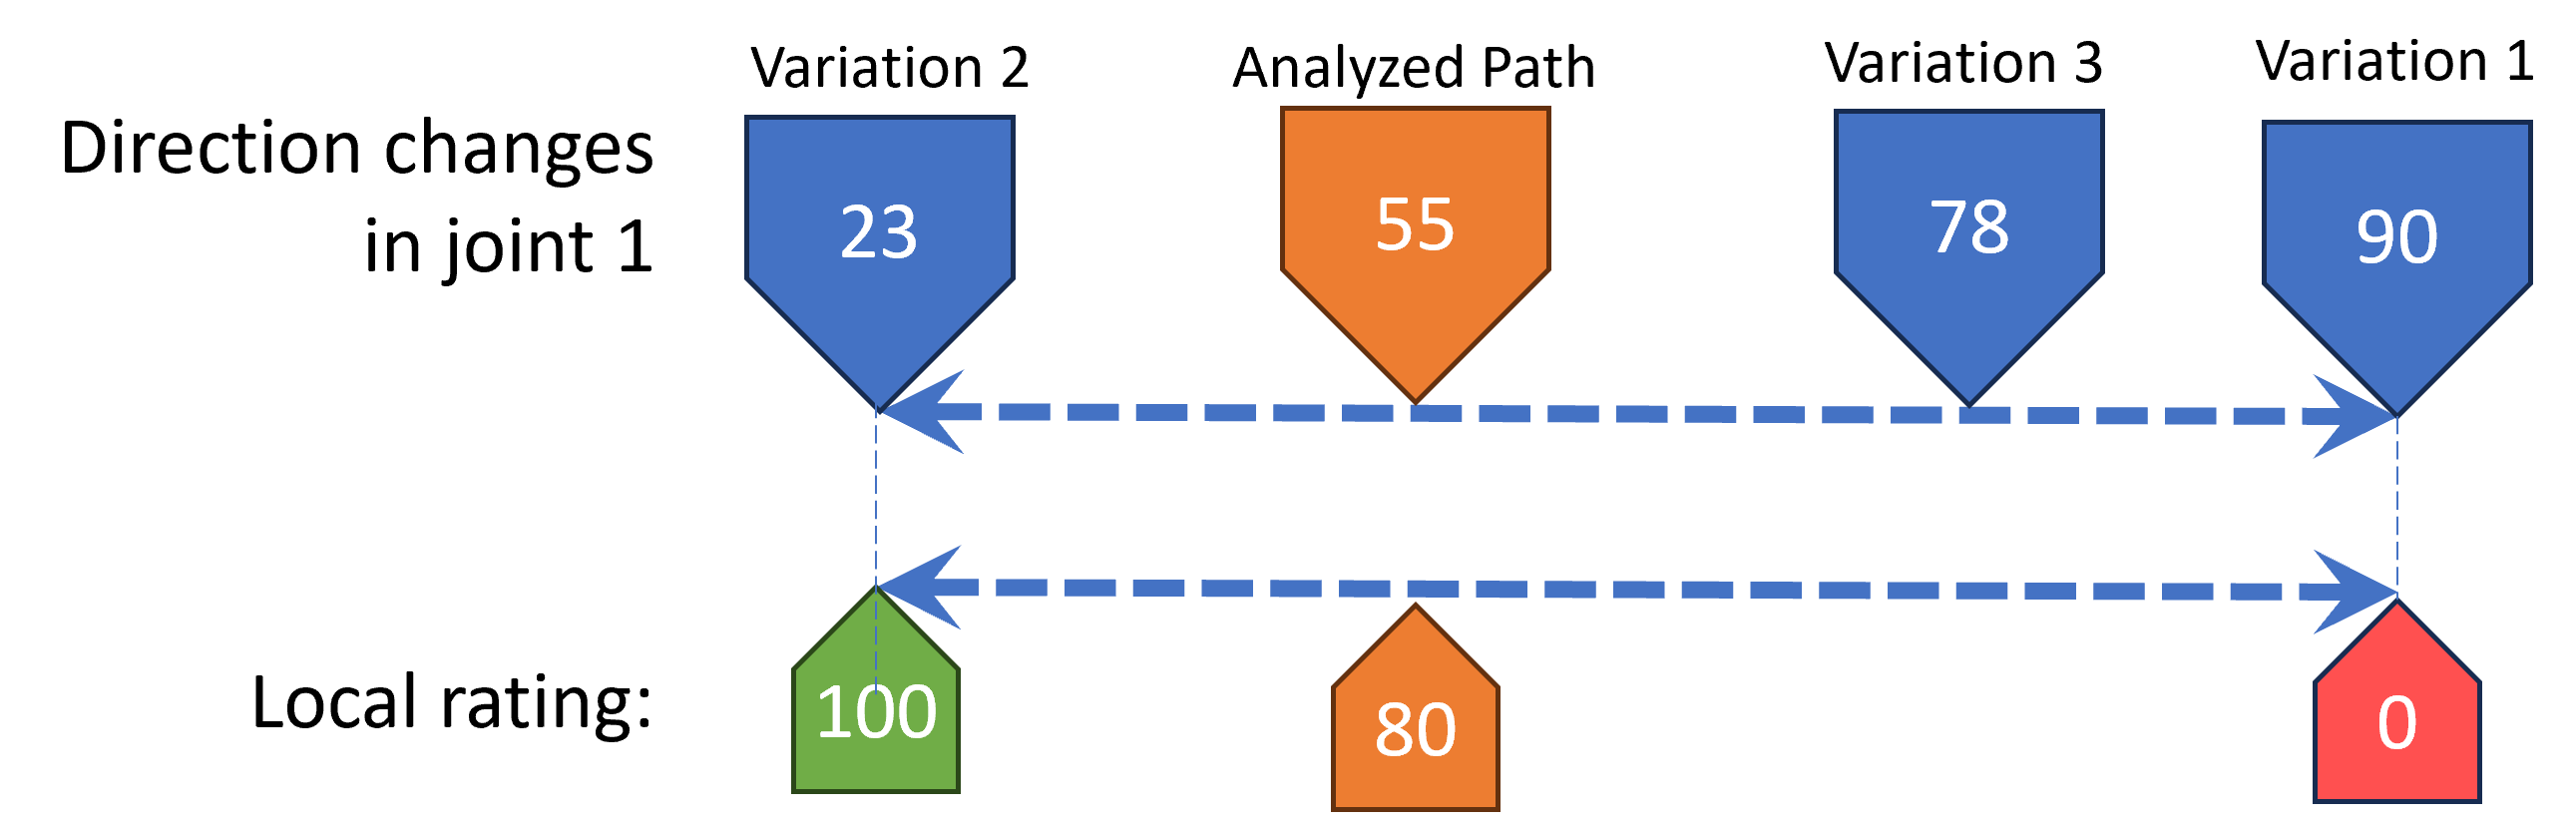
\includegraphics[scale=.6]{figures/localscore.png}}
	\caption{Calculation of the local score trough variation}
	\label{Localscore}
\end{figure}

Another factor that needs to be analyzed, is whether the variations in the results exceeds a certain standard deviation. Figure \ref{lowstd}, shows how a local score of 66 is calculated despite the presence of very small absolute differences. In this case, the standard deviation is only 0.37. Figure \ref{highstd} demonstrates how the same local score of 66 is calculated even though the absolute differences are significantly higher. Here, the standard deviation is 22.36.

Only if the standard deviation exceeds a set threshold, the local score should be calculated. In cases where the standard deviation criteria is not met the corresponding process parameter is omitted from the score calculation.

\begin{figure}[H]
	\centerline{\includegraphics[scale=.6]{figures/lowstd.png}}
	\caption{Variation with low standard deviation}
	\label{lowstd}
\end{figure}

\begin{figure}[H]
	\centerline{
\includegraphics[scale=.6]{figures/highstd.png}}
	\caption{Variation with high standard deviation}
	\label{highstd}
\end{figure}

 
\subsection{Information Extraction form Time-Series Data}\label{extraction}
It is important to note that for a local score computation as mentioned in Chapter \ref{LRC}, a time-series needs to be transformed into a scalar value. This can either be done by directly transforming the time series like for example summing up all values or performing a subsequent analysis. As each time series is capturing different phenomena, each one requires a individual process for transforming into a scalar value.

\section{Information from Angular Position}
The angular position of a joint by itself does not provide much information from which much qualitative analysis can be performed. But by adding information like a temporal component it can serve as a significant information source. 

Figure \ref{agularstuff} visualizes what information needs to be added to enhance the information content of process parameters that are directly related to the angular position of joints.

\begin{figure}[H]
	\centerline{\includegraphics[scale=.55]{figures/angularstuff.png}}
	\caption{Additional Information for angular position of each joint}
	\label{agularstuff}
\end{figure}



The first additional required information is the temporal element that specifies the time when a joint is supposed to be at what rotational position. This information can either be recorded in equidistant time steps as shown in figure \ref{equi} or adapted to only record the change of of position as shown in figure \ref{onchange}. Recording only the change of position is not optimal as it does not correspond the physical system where the position can not change from one time step to the other. Additionally it is no defined with which rotational velocity the joint need to change position. On the other hand, the continuous recording in equidistant time steps can result in significantly more recorded values and thus longer time-series.

Figure \ref{equi} shows the rotational position of a rotary joint in radians recorded with equidistant steps. Figure \ref{onchange} shows how a time-series looks like if only the destination positions and the associate times are recorded.

\begin{figure}[H]
	\centerline{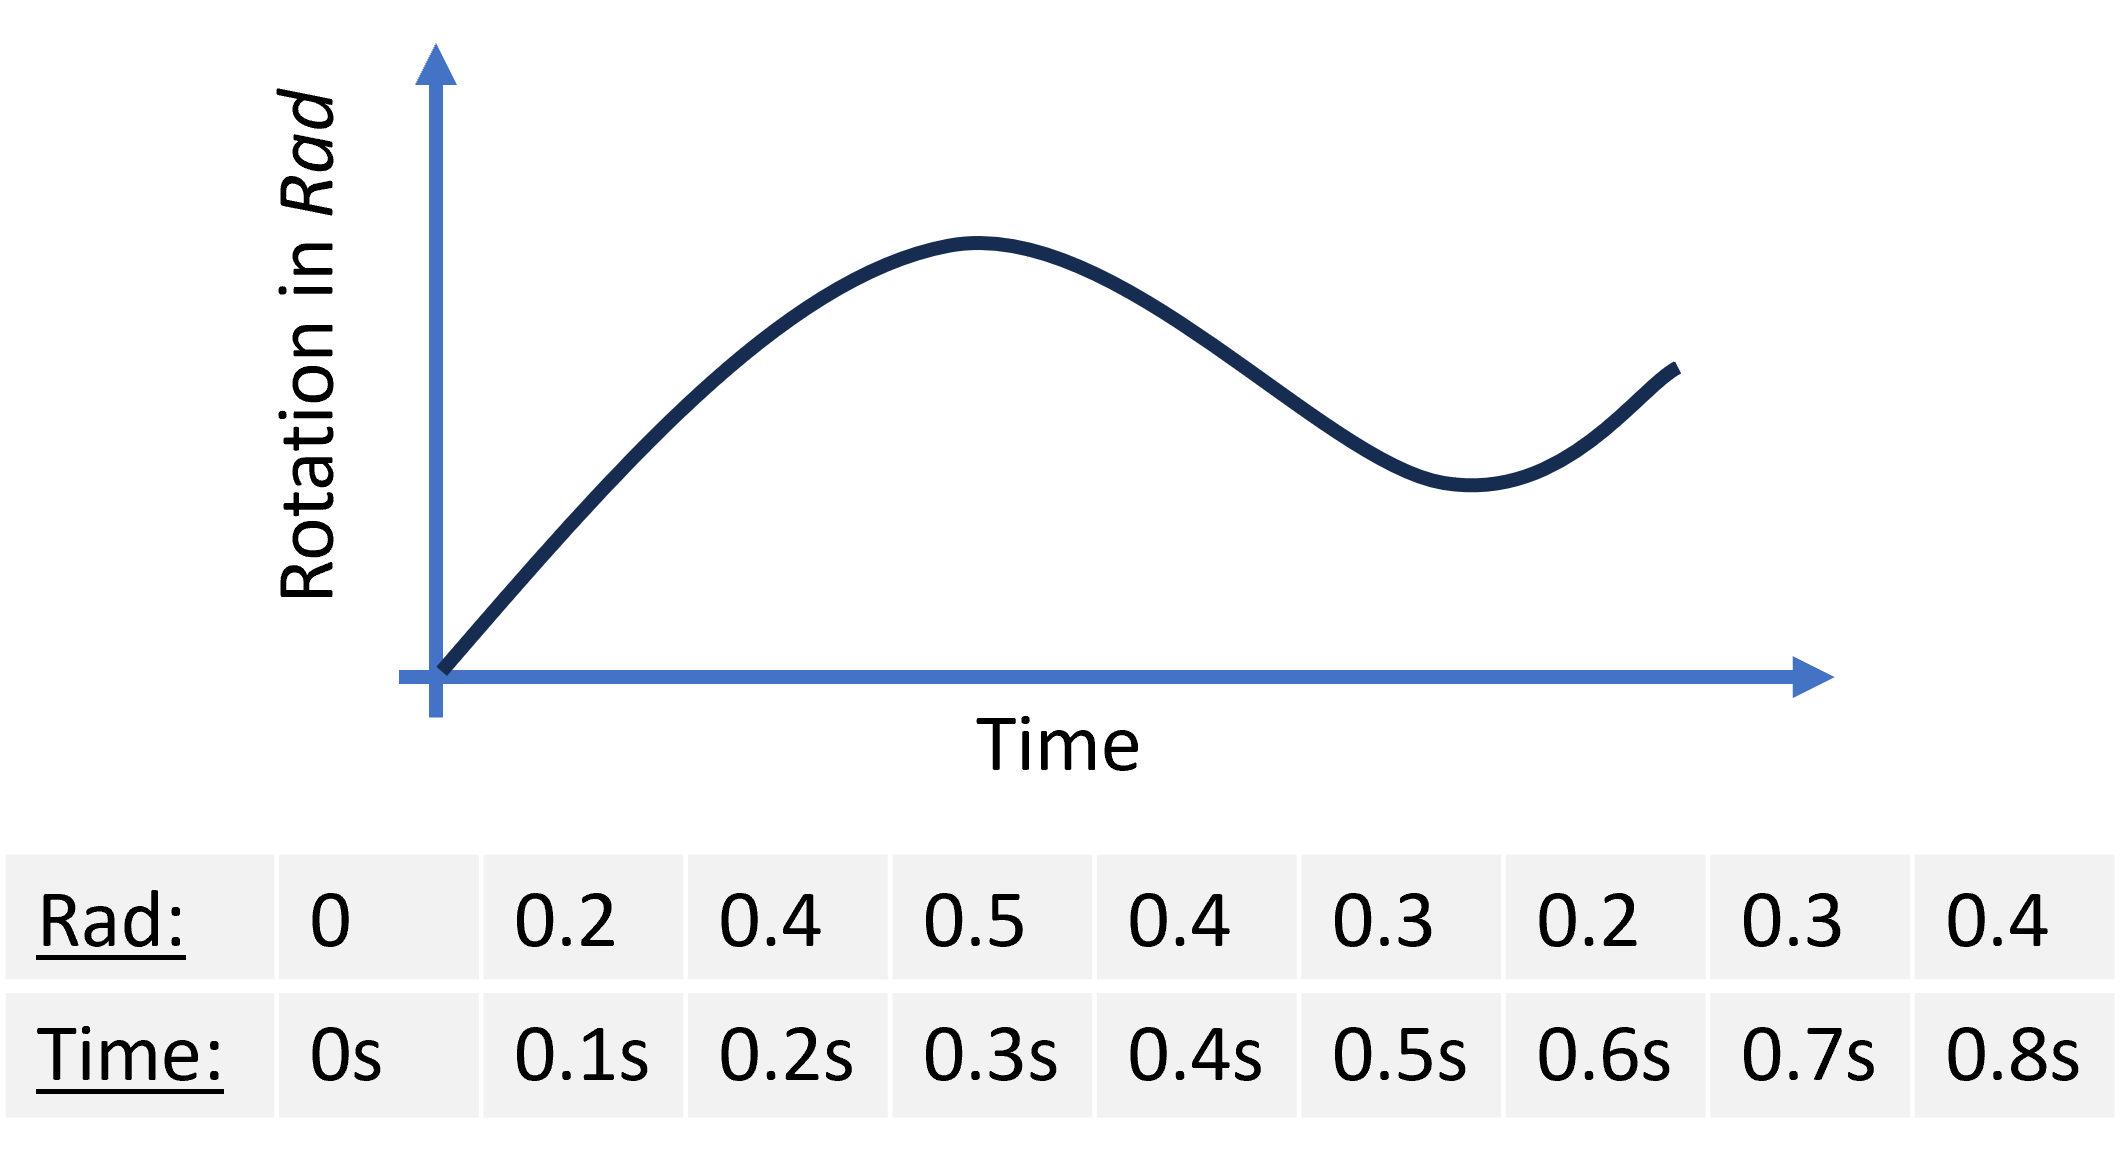
\includegraphics[scale=.6]{figures/equi.png}}
	\caption{Time-series of a rotary joint with equidistant time steps}
	\label{equi}
\end{figure}

\begin{figure}[H]
	\centerline{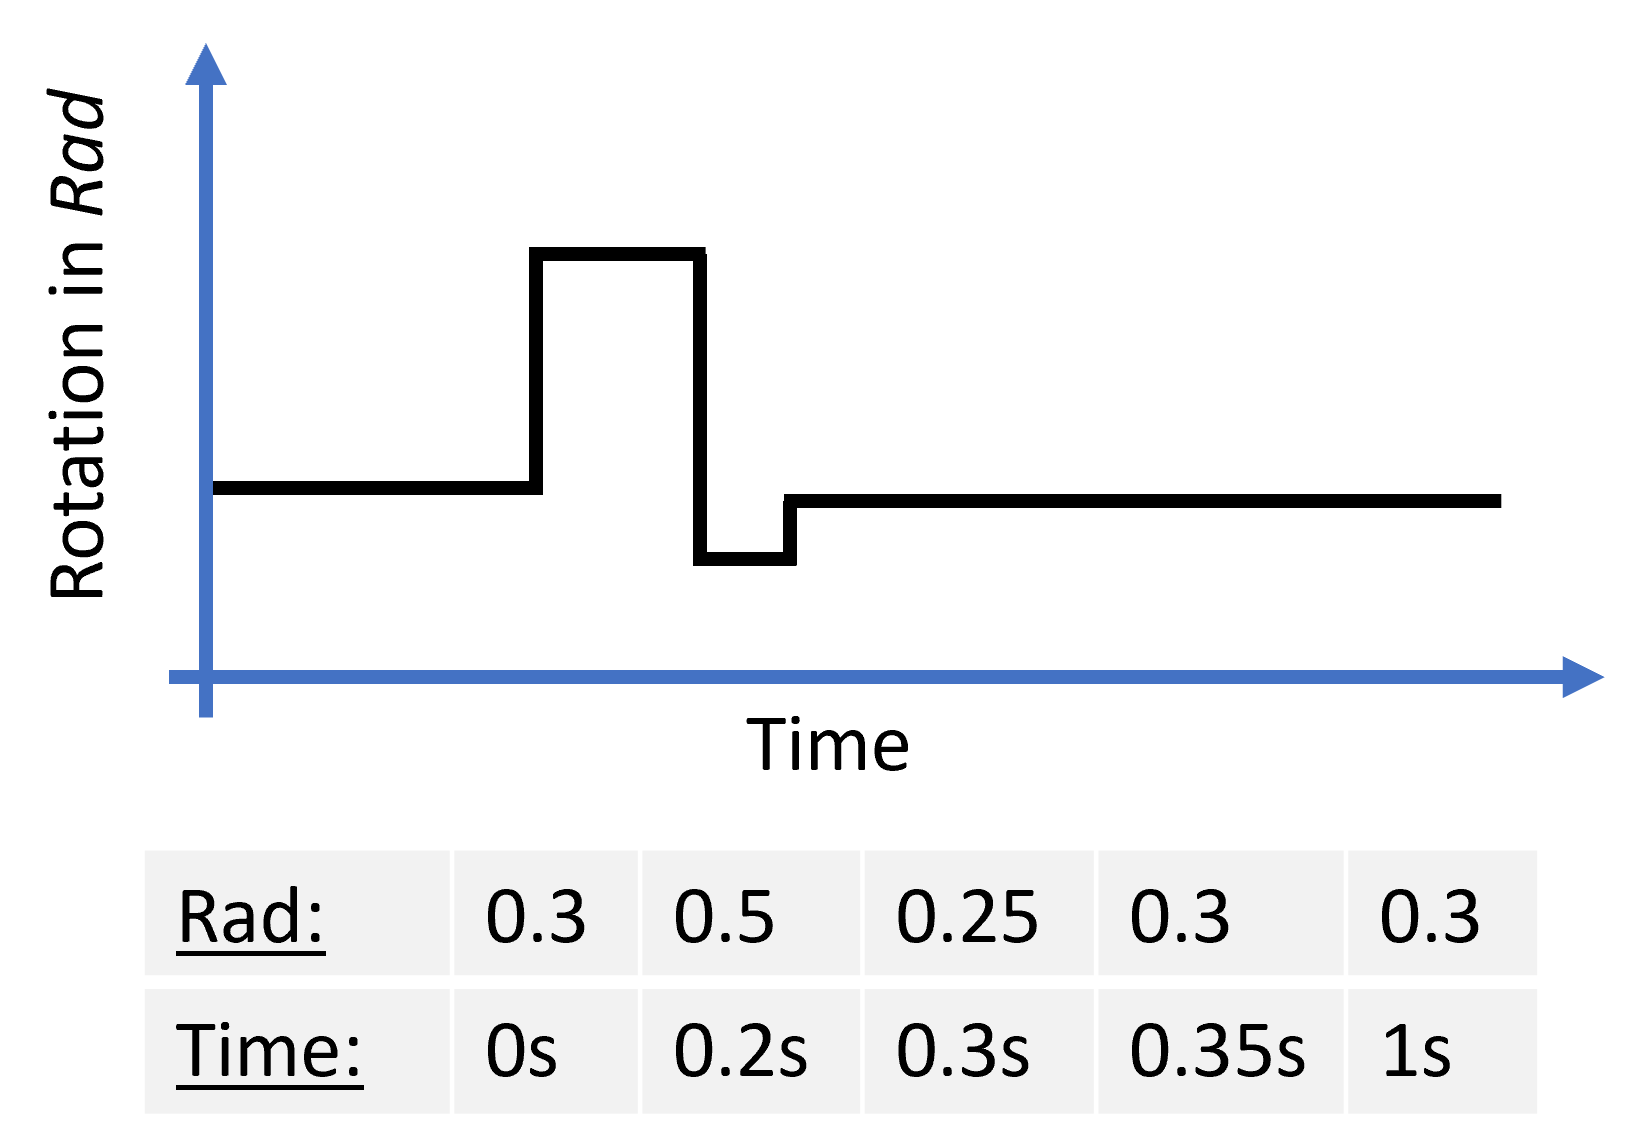
\includegraphics[scale=.6]{figures/onchange.png}}
	\caption{Time-series of a rotary joint with only the recorded end positions}
	\label{onchange}
\end{figure}

\subsection{Total Joint Travel}
Parameters that can be analyzed without any additional information is the number of direction changes as well as the total travel of a joint. The total travel is easily obtained by subtracting the position on two adjacent recorded points and summing up the absolute value. Additionally more information can be extracted by summing up, for example, the clockwise and anti-clockwise rotation individually. By combing the absolute value of these to values, the total travel of that joint is calculated.

Figure \ref{travel} gives a visual representation on how the total travel can calculated. Summing up the length of the green arrows result in the total forward rotation, while the sum of the length of the orange arrows is the backwards rotation.

\begin{figure}[H]
	\centerline{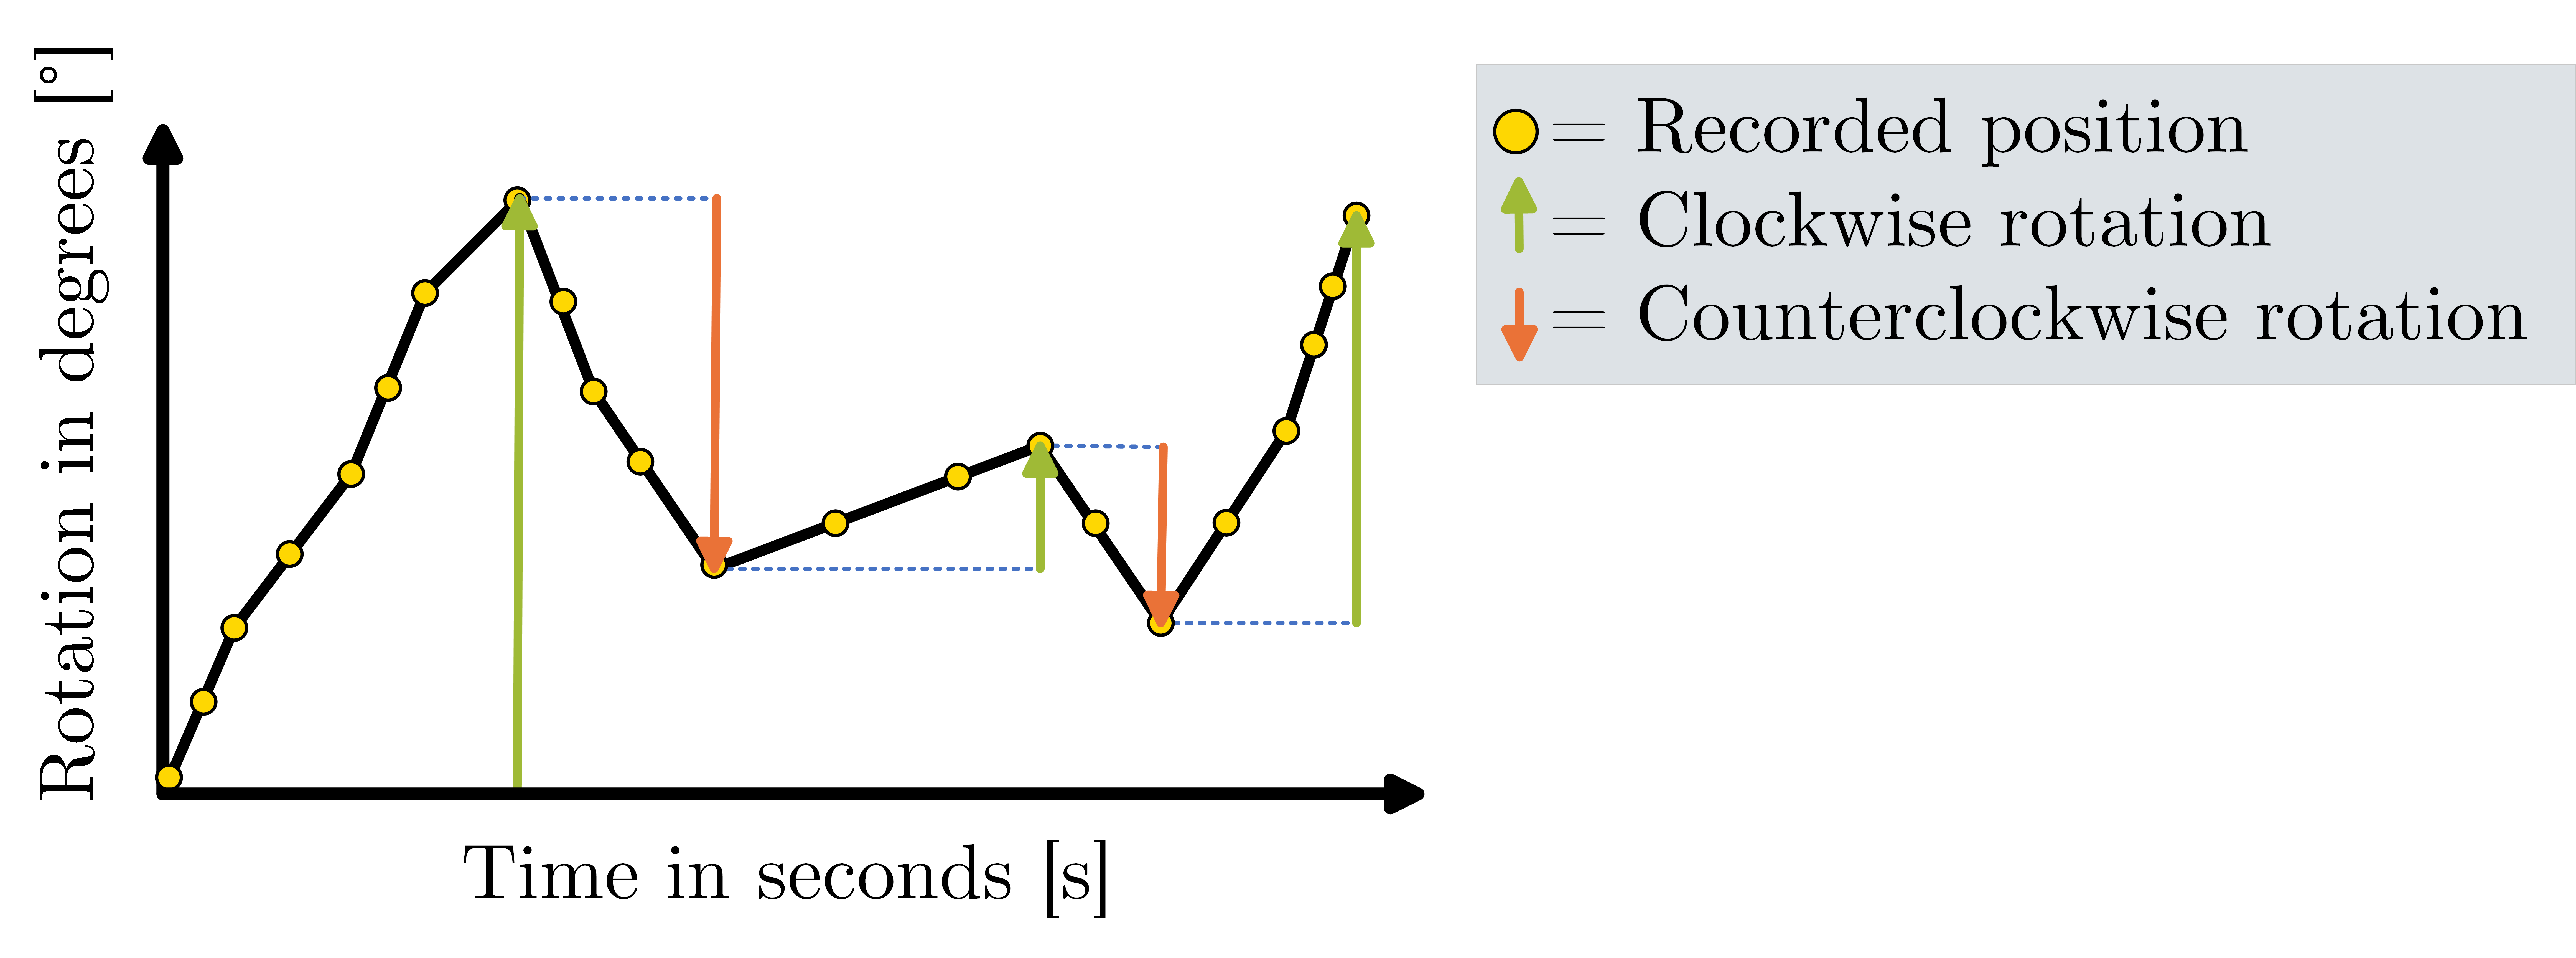
\includegraphics[scale=.6]{figures/travel.png}}
	\caption{Summing up the rotation in the clockwise and anti-clockwise direction }
	\label{travel}
\end{figure}

\subsection{Direction changes}
The number of direction changes can also be determined by just analyzing the joint position without temporal information. This value can be determined by finding all points where the position before and after is either smaller or larger. 
But this method does not apply to points where multiple positions are recorded at the same value right after each other. 

The solution to that problem is to introduce a tracking value that indicates if the previous change in direction of two adjacent positions was either up or down. If the direction of two positions is different form the tracking value, the direction change counter is incremented by 1. If the direction is in the same as the previous points or neutral, which means that two positions were identical, the direction change counter and tracking values is not changed.

Figure \ref{dirchange} gives a visual representation where the direction-change counter is incremented.

\begin{figure}[H]
	\centerline{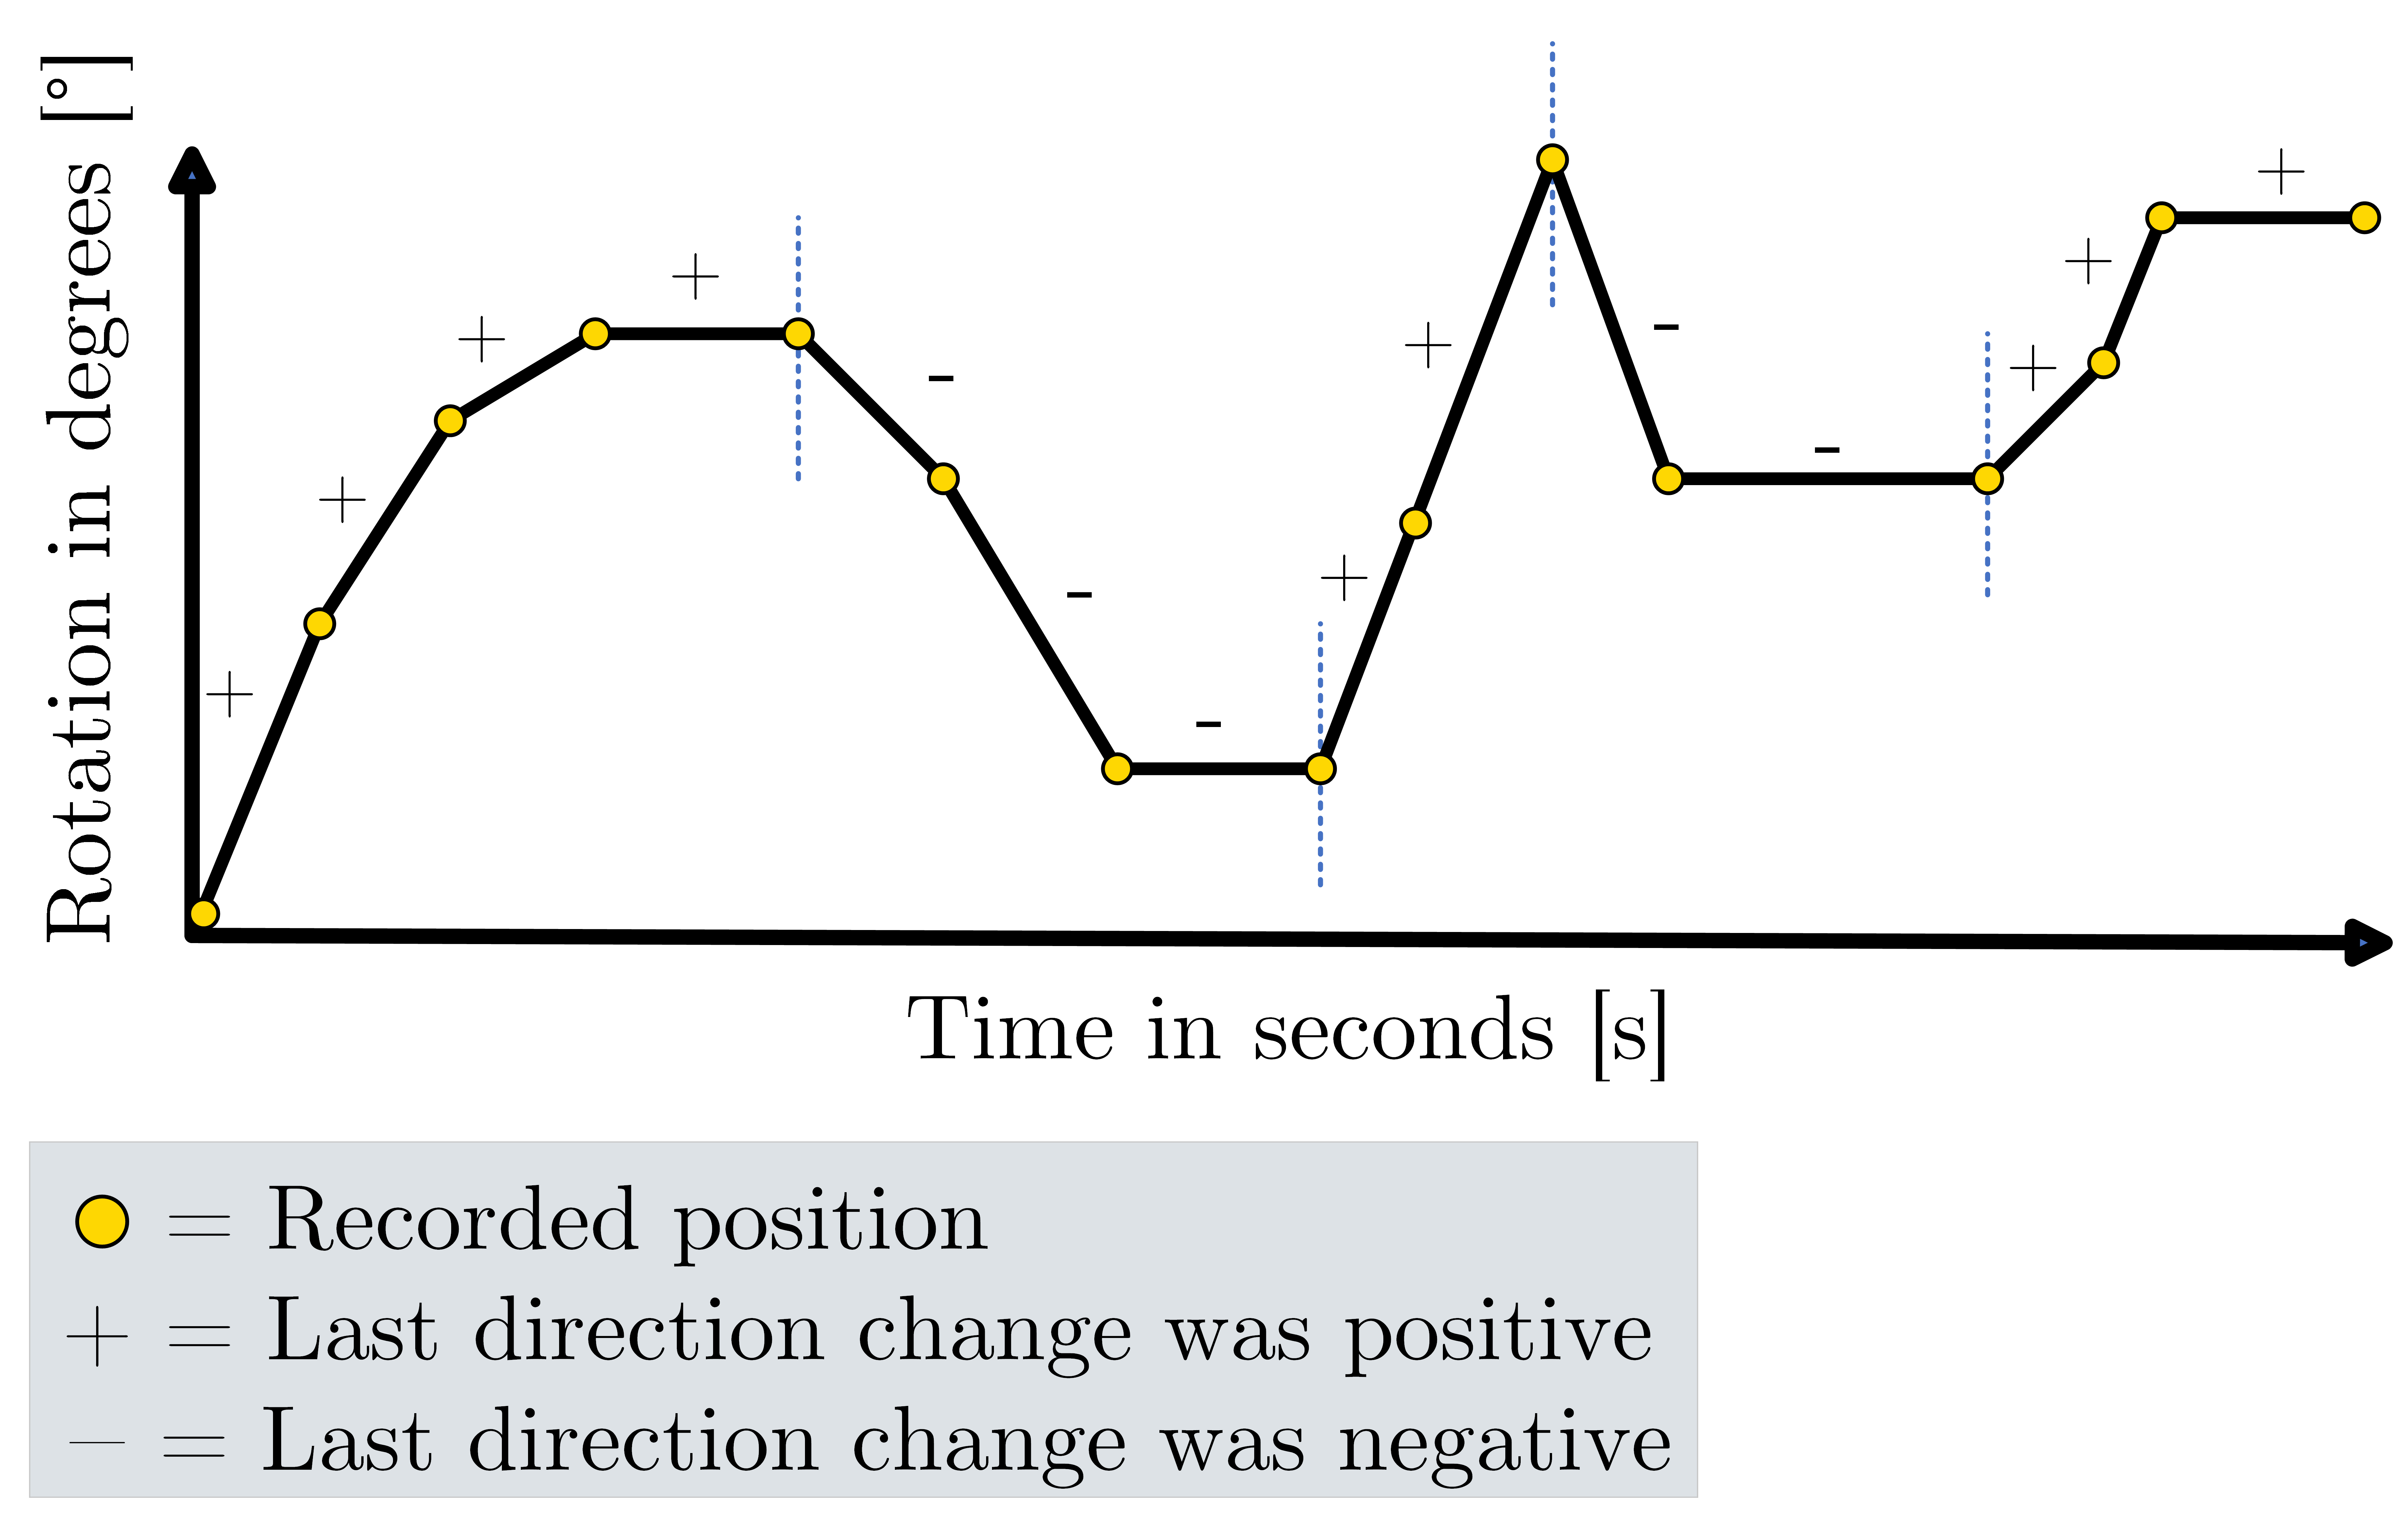
\includegraphics[scale=.55]{figures/dirchange.png}}
	\caption{Calculating direction changes from a time series}
	\label{dirchange}
\end{figure}

In some cases it is not possible to reduce the number of direction changes by adapting the boundary conditions. But having the same number of direction changes does not make two time series identical. Figure \ref{dirchangeSTD} shows how a two time series have the same number of direction changes but have significantly different characteristics. To differentiate these cases, a values corresponding to the standard deviation can be employed. Tool paths that result in frequent and temporally close positioned direction changes are generally not advisable.

\begin{figure}[H]
	\centerline{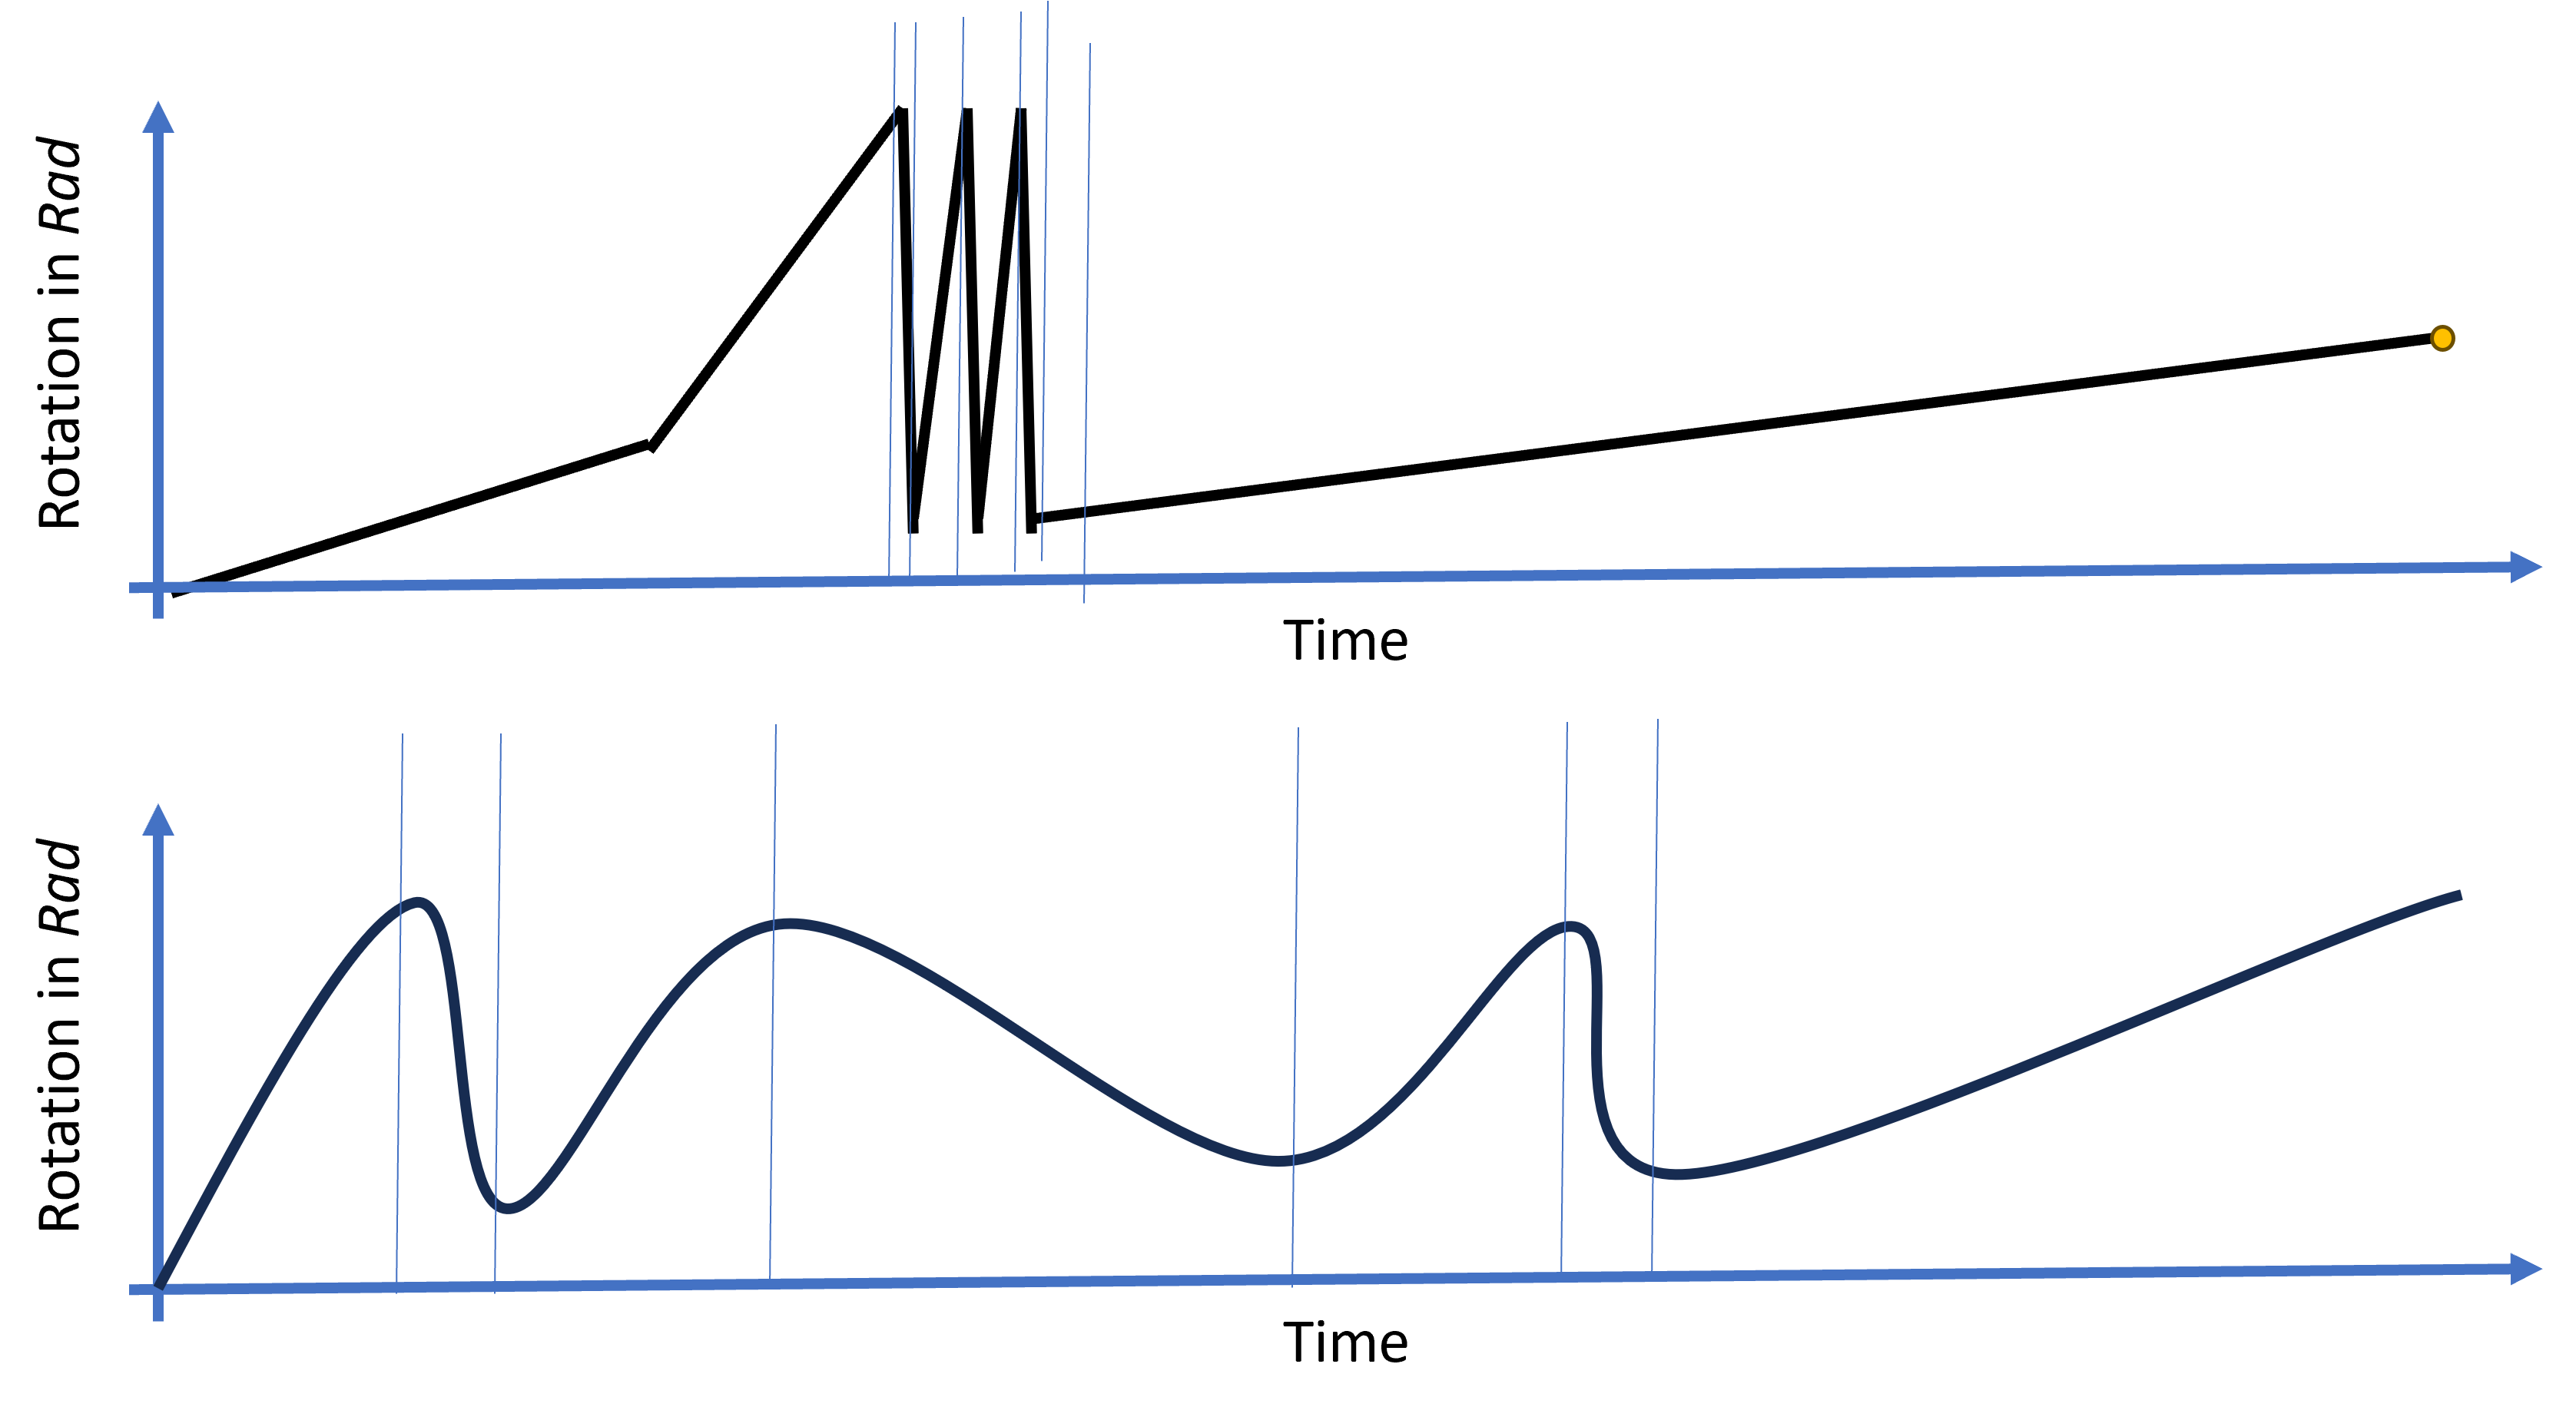
\includegraphics[scale=.4]{figures/DirSTD.png}}
	\caption{Standard Deviation direction changes from a time series}
	\label{dirchangeSTD}
\end{figure}

\subsection{Rotation Limits}
Lastly, a simple analysis regarding the rotational limits can be performed, for that two different values need to be known. The fist one is the physical limit that a joint can not exceed. Trying to drive the robot joint past that point can result in significant damage. The second value are possible soft limits that exist to prevent the joint from over rotation into its physical limits. To validate if any rotational positions come close to the limits or are exceeded, a simple comparison of all the values can be made.

\subsection{Velocity, Acceleration and Jerk}
To specifically analyze the velocity, acceleration and jerk a time derivative needs to be performed. After that simple comparisons of the time series values is enough to determine whether 
the maximum capabilities of the motor driving the joint are exceeded.


Figure \ref{velo} shows how the velocity aspect can be transformed into a scalar value that can be used as a local score. First, the joint velocity is obtained by taking a time derivative. Then it is analyzed for how long the absolute velocity exceeded a certain threshold value. In this case the threshold is set at 80\%. Further more it is possible to add multiple thresholds and weigh them exponentially in relation to each other. The combined result is then used as a local score. In the case that the velocity exceeds the maximum velocity, a "No-Go" exception must be thrown as that movement is not possible.
  
The absolute jerk 
\begin{figure}[H]
	\centerline{\includegraphics[scale=.5]{figures/veloy.png}}
	\caption{x}
	\label{velo}
\end{figure}

The same principle is applicable to the joint jerk. The duration the absolute jerk is over a threshold can be transformed into the local score, while exceeding the maximum possible jerk will trigger a "No-Go" exception.


ÜBERSWEIFEN
\section{Energy Usage}
\section{Reach, Singular, Torch Orientation}
\section{General Methodology for Process Optimization}